% !TEX root = Bachelorarbeit Synthetische Daten.tex
\chapter{Theoretische Grundlagen}

Das folgende Kapitel gibt eine Einführung in die theoretischen Grundlagen, die für das Verständnis der Arbeit notwendig sind. Dabei werden vor allem zentrale Konzepte und Methoden des maschinellen Lernens, der synthetischen Datengenerierung, sowie des Contrastive Learning behandelt. Zuletzt wird die Forschungslücke vorgestellt, die die Arbeit adressiert, und ein eigener Ansatz zur Integration von DA-Fusion und Supervised Contrastive Learning definiert.

\section{Maschinelles Lernen} \label{sec:ml}
	% KI-Einleitung?
	% Was geht ab bei dem goodfellow Zitat?

% Einleitung; KI als Herausforderung
Maschinelles Lernen (ML) ist als Teilgebiet der Künstlichen Intelligenz (KI) einzuordnen, einem interdisziplinären Forschungsfeld, das sich mit der Entwicklung von Algorithmen und Techniken befasst, welche es Computern ermöglichen, menschenähnliche Intelligenz zu erlangen.

% Ursprung ML; Problemstellung
Die ersten großen Durchbrüche in der KI kamen im Bezug auf Aufgaben, die für Menschen intellektuell eine große Herausforderung darstellten, die aber von Computern relativ einfach zu lösen waren, da sie als Liste formaler, mathematischer Regeln beschrieben werden konnten. Die große Schwierigkeit lag hingegen in den Aufgaben, die für Menschen relativ einfach und intuitiv sind, welche sich aber nur schwer formal beschreiben lassen. Hierunter fallen z.B. die Spracherkennung, oder Objekterkennung \parencite{Goodfellow2016deeplearning}.

Maschinelles Lernen beschreibt den Ansatz, Computer mit der Fähigkeit auszustatten, selbstständig Wissen aus Erfahrung zu generieren, indem Muster und Konzepte aus rohen Daten erlernt werden. So kann ein Computerprogramm auf Basis von Beispielen lernen, wie es eine bestimmte Aufgabe lösen soll, ohne dass ihm explizit Regeln oder Algorithmen vorgegeben werden.

% Definition ML (Mitchell), weiter ausgeführt
Eine allgemeine Definition für Maschinelles Lernen bietet \parencite{Mitchell1997machinelearning}:

\begin{quote}
	Ein Computerprogramm soll aus Erfahrung $E$ in Bezug auf eine Klasse von Aufgaben $T$ und Leistungsmaß $P$ lernen, wenn sich seine Leistung bei Aufgaben $T$, gemessen durch $P$, mit Erfahrung $E$ verbessert.
\end{quote}

Die Erfahrung $E$ besteht dabei aus einer Menge von Trainingsdaten, beispielsweise Bilder. Die Aufgaben $T$ können sehr unterschiedlich sein, von einfachen Klassifikations- und Regressionsaufgaben bis hin zu komplexen Problemen wie Spracherkennung oder autonomes Fahren. Das Leistungsmaß $P$ gibt an, wie gut die Aufgaben $T$ gelöst werden, und kann z.B. die sogenannte Accuracy sein, welche den Anteil korrekt klassifizierter Beispiele angibt.

Durch das Lernen aus den Trainingsdaten ergibt sich ein \textit{Modell} des zugrundeliegenden Problems, das dann auf neue, unbekannte Daten angewendet werden kann, um Vorhersagen zu treffen oder Entscheidungen zu treffen.

\subsection{Überwachtes und unüberwachtes Lernen} \label{sec:sup-unsup}

% Supervised & Unsupervised als die zwei wichtigsten Lernparadigmen im ML
Wie genau Wissen aus Erfahrung bzw. aus Rohdaten generiert wird hängt vom gewählten Verfahren ab. Im Maschinellen Lernen gibt es dabei zwei zentrale Paradigmen, das überwachte und das unüberwachte Lernen.

% Supervised
Beim überwachten Lernen (Supervised Learning) wird das Modell mit einem vollständig annotierten Datensatz trainiert. Das heißt meistens, dass jeder Datenpunkt mit einem Klassenlabel versehen ist, sodass Eingabe-Ausgabe-Paare entstehen. Ziel ist es, eine Funktion zu lernen, welche die Eingaben auf die entsprechenden Ausgaben abbildet. Ein einfaches Beispiel wäre ein Bildklassifikator, der darauf trainiert wird, Katzen und Hunden zu unterscheiden. Hier würden alle Trainingsbilder entweder mit dem Label „Katze“ oder „Hund“ versehen sein. Im Training kann die Vorhersage des Modells dann mit dem tatsächlichen Label verglichen werden, um den Fehler zu berechnen und die Modellparameter entsprechend anzupassen.

% Unsupervised
Im Gegensatz dazu arbeitet unüberwachtes Lernen (Unsupervised Learning) mit unbeschrifteten Daten; es gibt also keine vorgegebenen Ausgaben. Stattdessen wird versucht, ein Modell zu befähigen, eigenständig Muster und Strukturen in den Daten zu erkennen und z.B. nützliche Repräsentationen der Eingangsdaten zu erlernen. Zu den häufigsten Methoden des unüberwachten Lernens gehören Clustering- und Assoziationsalgorithmen. Ein Beispiel ist die Segmentierung von Kunden in verschiedene Gruppen basierend auf ihrem Kaufverhalten \parencite{}.

% Andere; Semi-supervised & Self-supervised
In der Praxis werden oft auch hybride Ansätze genutzt, wie das semi-überwachte Lernen (Semi-Supervised Learning), bei dem eine Kombination aus beschrifteten und unbeschrifteten Daten verwendet wird, oder das selbstüberwachte Lernen (Self-Supervised Learning), bei dem das Modell eigenständig Teile der Daten zur Erzeugung von Überwachungssignalen verwendet, anstatt sich auf externe, von Menschen bereitgestellte Labels zu verlassen.

\subsection{Deep Learning} \label{sec:deep-learning}

% Eine Hierarchie von Konzepten
Das Wissen, das ein Modell aus den Trainingsdaten lernt, wird in Form von sogenannten Features repräsentiert. Diese Features können einfache Konzepte wie Kanten oder Farben sein, oder komplexere Konzepte wie Gesichter oder Objekte. Unter Deep Learning (DL) versteht man eine tiefe, hierarchische Vernetzung dieser Konzepte, sodass komplexere Konzepte auf simpleren Konzepten aufbauen können. Visuell veranschaulicht entsteht ein Graph mit vielen Ebenen, oder \textit{Deep Layers} \parencite{Goodfellow2016deeplearning}.

% Unterkategorie des ML
Deep Learning ist also eine Unterkategorie des Maschinellen Lernens (siehe Abbildung \ref{fig:ai-venn}), bei der die Eingabedaten mehrere Verarbeitungsschichten durchlaufen, um eine hierarchische Repräsentation zu ermöglichen. Jede Schicht transformiert die Eingabedaten in eine etwas abstraktere Darstellung. Deep Learning fällt demnach auch unter den Begriff des Representation Learning \parencite{Zhou2021machinelearning}.

\begin{figure}[t]
	\centering
	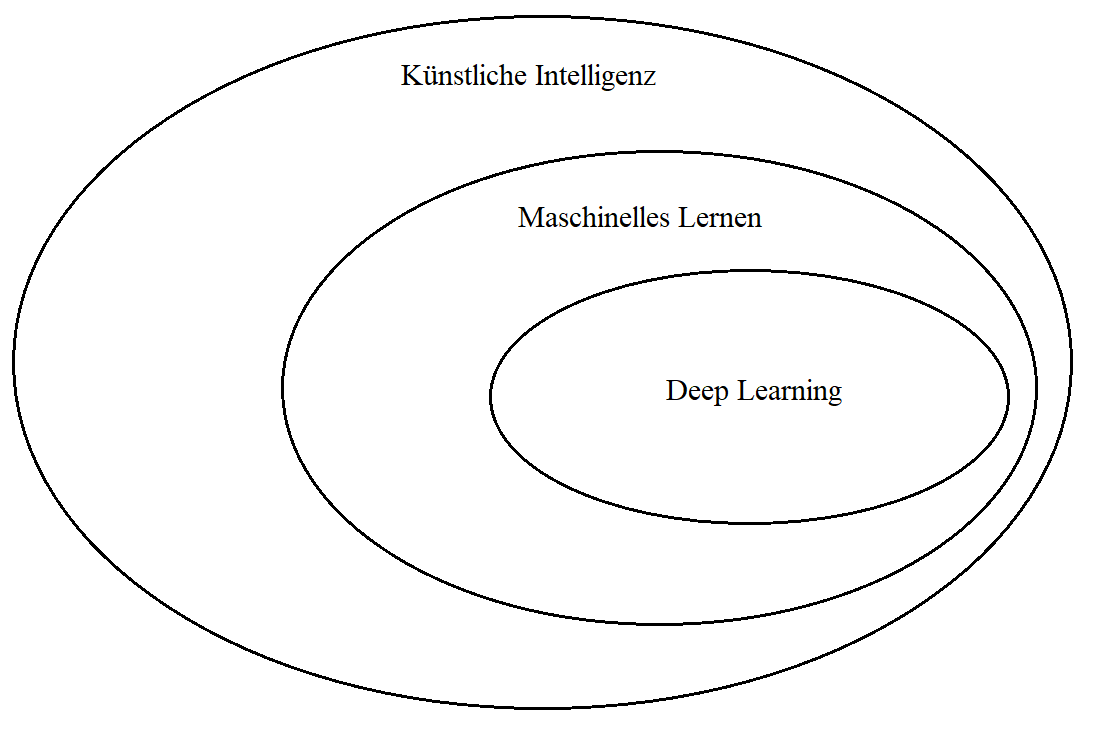
\includegraphics[width=12cm]{figure_ai_venn-diagram.png}
	\caption{Ein einfaches Venn-Diagramm, das die Beziehung zwischen KI,\\
	ML und DL veranschaulicht.}
	\label{fig:ai-venn}
\end{figure}

Heutzutage bilden Deep Learning-Modelle die Grundlage für viele Anwendungen der Künstlichen Intelligenz, darunter Bild- und Spracherkennung, maschinelle Übersetzung, medizinische Diagnose und autonomes Fahren. Die rasante Entwicklung in diesem Bereich ist vor allem auf die Verfügbarkeit großer Datenmengen und immer leistungsfähigere Hardware zurückzuführen \parencite{Goodfellow2016deeplearning}. %?

\subsection{Neuronale Netze} \label{sec:neural-networks}

% Einleitung und grundlegender Aufbau
Während die rasante Entwicklung von Deep Learning vor allem in den vergangenen Jahren spürbar geworden ist, sind die zugrundeliegenden Algorithmen und Konzepte schon seit Jahrzehnten bekannt \parencite{Zhou2021machinelearning}. Dabei bildet das künstliche neuronale Netz (KNN) die Grundlage der allermeisten Deep-Learning-Modelle. Es ist inspiriert von der Struktur und Funktionsweise des menschlichen Gehirns und besteht aus einer Vielzahl von miteinander verbundenen Knoten (Neuronen), die in Schichten organisiert sind. Die Struktur eines neuronalen Netzes besteht aus einer Eingabeschicht (Input Layer), einer oder mehreren versteckten Schichten (Hidden Layers) und einer Ausgabeschicht (Output Layer). %, wie in Abbildung \ref{fig:ffn} dargestellt.

%\begin{figure}[t]
%	\centering
%	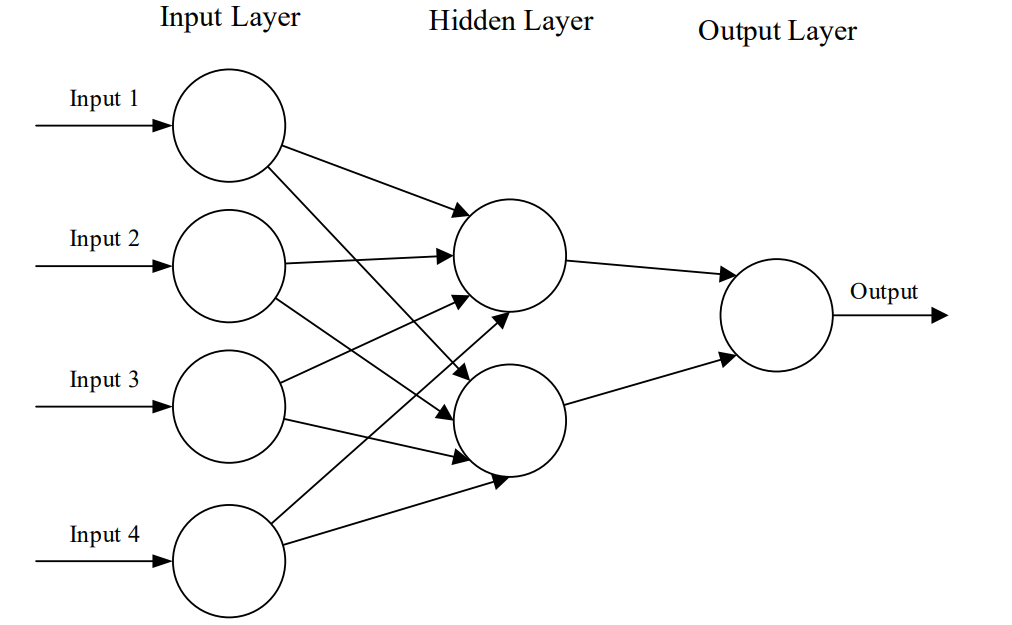
\includegraphics[width=11cm]{figure_ffn.png}
%	\caption{Darstellung eines einfachen neuronalen Netzes \parencite{Oshea2015cnnintro}.}
%	\label{fig:ffn}
%\end{figure}

% Einzelnes Neuron im Detail
Die einzelnen Neuronen, auf dem diese Netze aufbauen, sind eine mathematische Modellierung des biologischen Neurons, das erstmals 1943 von Warren McCulloh und Walter Pitts vorgestellt wurde \parencite{Zhou2021machinelearning}. In Abbildung \ref{fig:neuron} ist das Modell dargestellt.

\begin{figure}[h]
	\centering
	\vspace*{4mm}
	%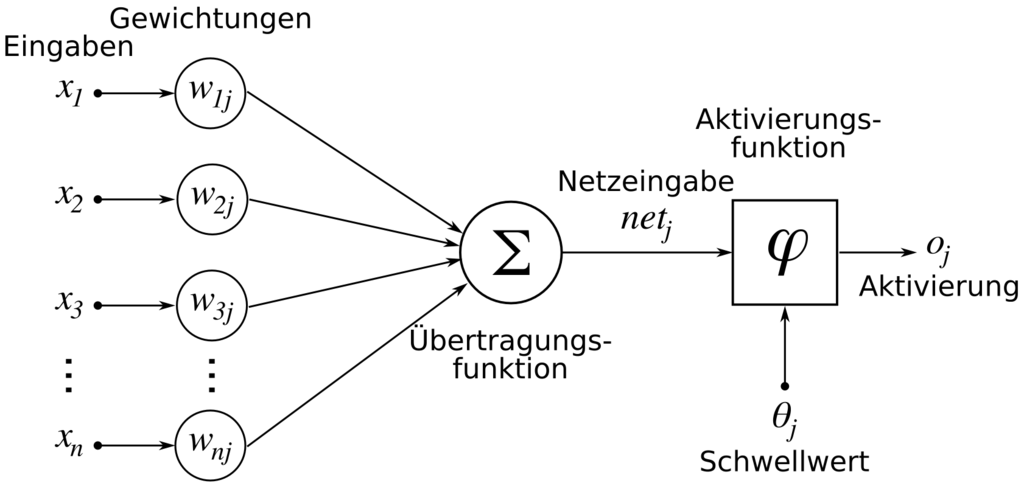
\includegraphics[width=12cm]{figure_mp-neuron.png} % https://commons.wikimedia.org/w/index.php?curid=224561
	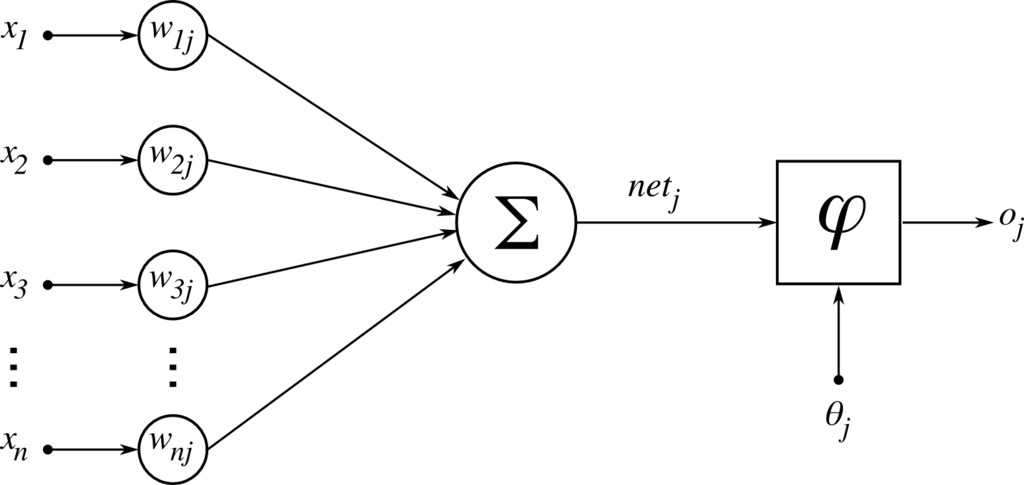
\includegraphics[width=12cm]{figure_mp-neuron_nd.png} % https://commons.wikimedia.org/wiki/File:ArtificialNeuronModel.png
	\vspace*{2mm}
	\caption{Das McCulloch-Pitts-Modell eines Neurons.}
	\label{fig:neuron}
\end{figure}

Jedes Neuron empfängt eine Reihe von Eingaben $x_{1 \dots n}$, entweder von externen Quellen oder von den Ausgaben anderer Neuronen. Für jede dieser Eingaben gibt es zugehörige Gewichtungen (Weights) $w_{1j \dots nj}$, welche die Stärke und Richtung (positiv oder negativ) des Einflusses der jeweiligen Eingaben auf das Neuron $j$ bestimmen. Das Neuron berechnet dann die gewichtete Summe $net_j$ aller Eingaben und falls ein bestimmter Schwellenwert (Bias) $\theta$ überschritten wurde, wird das Neuron aktiviert. Die Aktivierung $o_j$ des Neurons kann dementsprechend folgendermaßen beschrieben werden:

\begin{equation}
	o_j = \phi \left( \sum_{i=1}^{n} w_i x_i - \theta_j \right)
	\label{eq:mp-neuron}
\end{equation}

% Aktivierungsfunktionen; Sigmoid & Softmax
Die Aktivierungsfunktion $\phi$ kann dabei unterschiedlich gewählt werden, um die Ausgabe des Neurons zu modellieren. Eine simples Beispiel ist die sogenannte Schwellenwertfunktion, die den Wert 1 zurückgibt, wenn die gewichtete Summe größer als der Schwellenwert ist, sonst 0. Eine häufig verwendete Aktivierungsfunktion ist jedoch die sogenannte Sigmoid-Funktion, die kontinuierlich und differenzierbar ist und somit die Optimierung des Netzwerks vereinfacht:

\begin{equation}
	\text{Sigmoid}(x) = \frac{1}{1 + e^{-x}}
	\label{eq:sigmoid}
\end{equation}

Während die Sigmoid-Funktion allerdings nur für binäre Klassifikationen geeignet ist, wird für die Klassifikation von mehreren Klassen die Softmax-Funktion verwendet, die die Wahrscheinlichkeitsverteilung über alle Klassen berechnet:

\begin{equation}
	\text{Softmax}(x)_i = \frac{e^{x_i}}{\sum_{j=1}^{n} e^{x_j}}
	\label{eq:softmax}
\end{equation}

% Wie neuronale Netze lernen; Loss-Funktionen, Backpropagation, Stochastic Gradient Descent
Im Training fließen die Eingabedaten in einer Vorwärtsausbreitung (Forward Propagation) durch das Netzwerk, um die Ausgabe zu berechnen. Es wird dann eine geeignete Verlustfunktion angewendet, um den Fehler (Loss) des Modells zu berechnen. Das Ziel des Trainings ist es, die Gewichtungen der Neuronen so anzupassen, dass der Fehler minimiert wird.

Diese Optimierung geschieht durch eine Rückwärtsausbreitung (Backpropagation), welche den berechneten Fehler rückwärts durch das Netz propagiert, um die Gewichte und Schwellenwerte um einen geringen Wert in die Richtung anzupassen, die den Fehler minimieren würde. Die Richtung wird bestimmt, indem der Gradient der Verlustfunktion berechnet wird. So bewegt sich das Modell iterativ entlang des Gradienten hin zu einem lokalen Minimum der Verlustfunktion. Dieser Algorithmus wird als Gradient Descent (Gradientenabstieg) bezeichnet. Im Maschinellen Lernen kommt jedoch hauptsächlich der Stochastic Gradient Descent (SGD) zum Einsatz, der immer nur einen kleinen, zufällig ausgewählten Teil der Trainingsdaten (einen sogenannten Batch) verwendet, um den Gradienten zu berechnen. %Goodfellow2016deeplearning?

% Hyperparameter
Es gibt eine Reihe von sogenannten Hyperparametern, welche einen großen Einfluss auf die Leistung des Modells haben und vorher manuell konfiguriert werden, oftmals durch Ausprobieren verschiedener Werte. Die Lernrate (Learning Rate) bestimmt beispielsweise, wie groß die Schritte sind, die entlang des Gradienten gemacht werden, während die Batch-Größe (Batch Size) die Anzahl der Trainingsdaten bestimmt, die in einem Schritt des SGD verwendet werden. Die Anzahl der Epochen gibt an, wie oft der gesamte Trainingsdatensatz durchlaufen wird. Andere Hyperparameter, wie die Anzahl der versteckten Schichten und Neuronen, bestimmen die Komplexität des Modells.

% CNN als Beispiel eines Deep Learning-Modells
\begin{figure}[h]
	\centering
	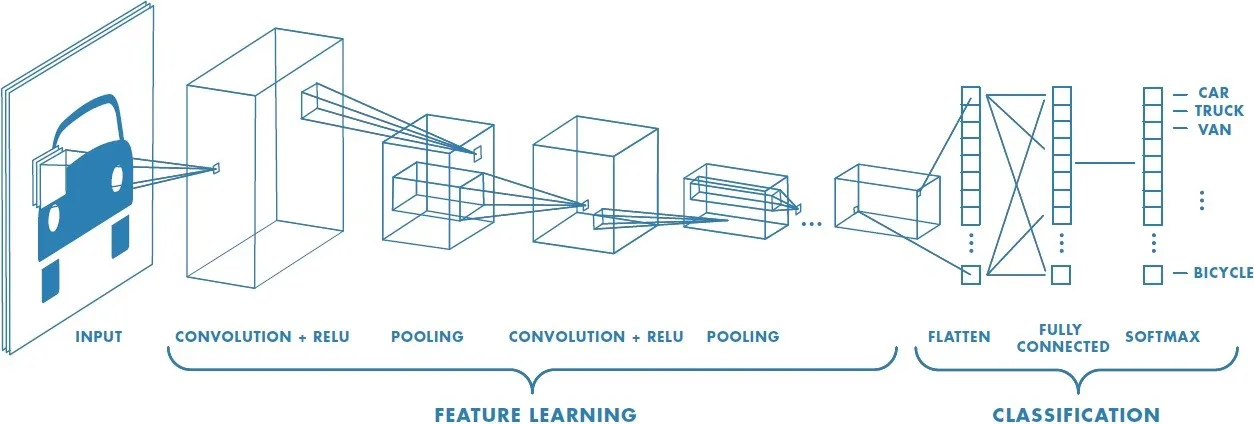
\includegraphics[width=\textwidth]{figure_cnn.png} % https://towardsdatascience.com/a-comprehensive-guide-to-convolutional-neural-networks-the-eli5-way-3bd2b1164a53
	\caption{Aufbau eines Convolutional Neural Networks (CNN)}
	\label{fig:cnn}
\end{figure}

% CNN als Deep Learning-Beispiel eines NN
Deep Learning mit neuronalen Netzen kann gut am Beispiel des Convolutional Neural Networks (CNN) veranschaulicht werden, welches speziell für die Verarbeitung von Bildern entwickelt wurde (siehe Abbildung \ref{fig:cnn}). Ein CNN besteht aus mehreren Schichten, darunter Convolutional Layers, Pooling Layers und Fully Connected Layers. Die Convolutional Layers extrahieren sogenannte \textit{Feature Maps} aus den Eingabebildern, indem sie Faltungskerne über das Bild schieben und die gewichteten Summen der Pixel berechnen. Die Pooling Layers reduzieren die Dimensionalität der Feature Maps, indem sie die Größe der Merkmale reduzieren. Die Fully Connected Layers kombinieren die extrahierten Merkmale, um die endgültige Klassifikation vorzunehmen.

Mit Backpropagation trainierte CNNs wurden erstmals in \parencite{LeCun1989cnnbackprop} behandelt, bilden aber auch heute noch die Grundlage von zahlreichen Deep Learning-Anwendungen und Methoden. Sie sind vor allem deshalb so erfolgreich in der Bildverarbeitung, weil sie die räumliche Struktur von Bildern berücksichtigen und dadurch eine hohe Genauigkeit bei der Klassifikation erreichen können.

\subsection{Overfitting} \label{sec:overfitting}

Wenn ein Modell so stark an die Trainingsdaten angepasst wird, dass es nicht in der Lage ist, auf neuen, unbekannten Daten zu generalisieren, spricht man von Overfitting \parencite{Goodfellow2016deeplearning}. Statt die zugrundeliegenden Muster zu lernen, speichert das Modell auch zufällige Rauschsignale und Fehler. Dies führt dazu, dass das Modell auf den Trainingsdaten eine hohe Genauigkeit erreicht, aber auf neuen Daten eine schlechtere Leistung zeigt. Man verwendet daher neben den Trainingsdaten auch Validierungsdaten zur Überwachung des Overfittings.

Oftmals liegt das Problem in der Quantität und Qualität der Trainingsdaten. Sind nicht genügend Daten vorhanden, oder sind die Daten nicht divers genug, kann das Modell nicht generalisieren.

Ein anderer Grund für Overfitting kann eine zu hohe Komplexität des Modells sein, wodurch die Trainingsdaten zu genau modelliert werden. Techniken zur Regularisierung zielen deshalb darauf ab, die optimale Komplexität eines Modells zu finden. Dropout \parencite{Srivastava2014dropout} ist eine solche Technik, bei der zufällig ausgewählte Neuronen während des Trainings deaktiviert werden, um zu verhindern, dass das Modell sich auf spezifische Merkmale verlässt. Als Early Stopping wird ein anderer Ansatz bezeichnet, bei dem das Training beendet wird, wenn die Leistung auf den Validierungsdaten beginnt, sich zu verschlechtern.

\subsection{Datenaugmentation} \label{sec:data-augmentation}

% Definition und Zweck
Datenaugmentation ist einer der wichtigsten Ansätze zur Vermeidung von Overfitting und findet in fast allen Methoden des Maschinellen Lernens Anwendung. Denn das Modell kann auch ohne völlig neue Daten zu beschaffen robuster gegenüber Variationen gemacht werden, indem es mit leicht veränderten Versionen der Trainingsdaten trainiert wird.

Bei der Datenaugmentation werden unterschiedliche Transformationen auf die vorhandenen Daten angewendet, z.B. Rotation, Skalierung, Verschiebung, Spiegelung, Helligkeitsanpassung oder Rauschen \parencite{Shorten2019dataaugmentation}. Die Transofrmationen werden meist mit zufälligen parametrisiert, um eine Vielzahl von Variationen zu erzeugen. Das Ziel ist es, das Modell zu zwingen, die zugrundeliegenden Muster der Daten zu lernen, anstatt sich auf spezifische Merkmale zu verlassen, die nur in den Trainingsdaten vorhanden sind. Einige Beispiele für Datenaugmentationstechniken sind in Abbildung \ref{fig:data-augmentation} dargestellt.

% Beispiele
\begin{figure}[h]
	\centering
	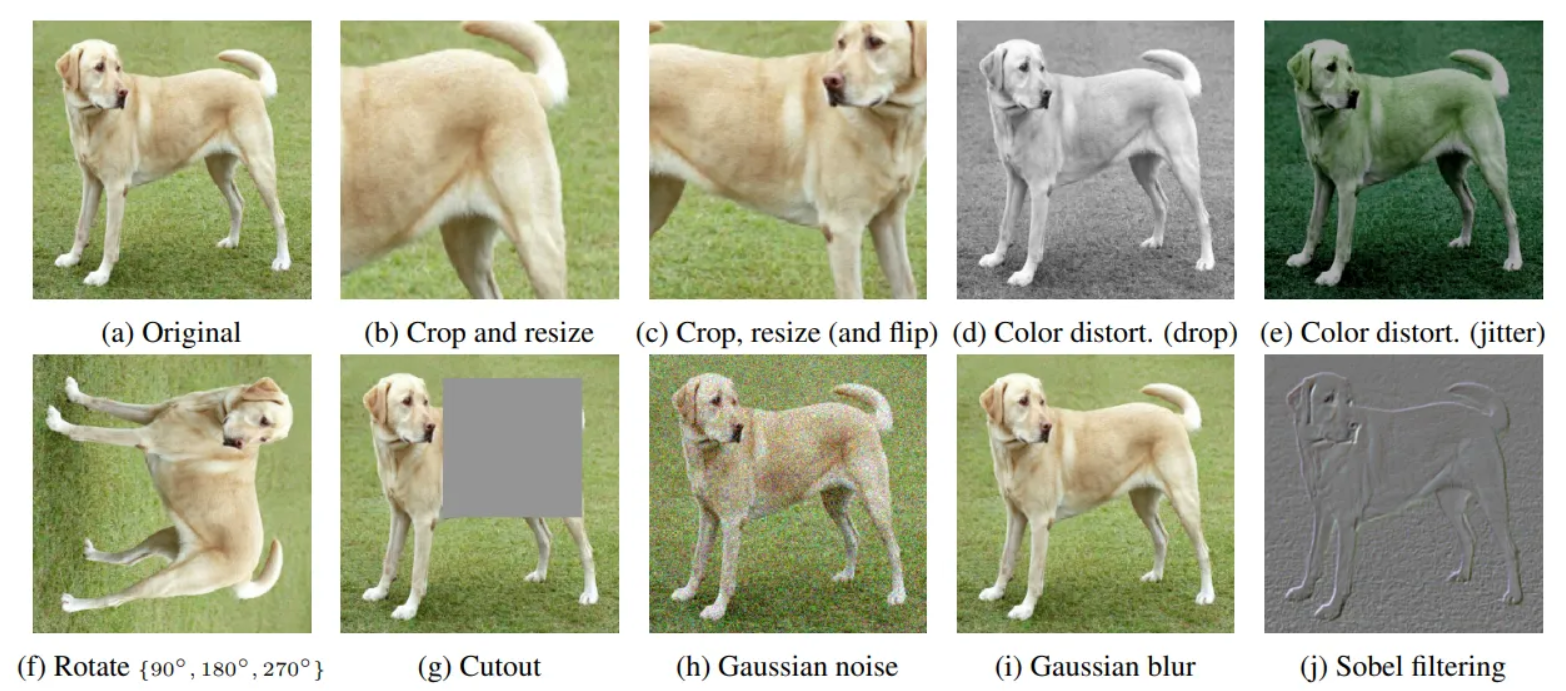
\includegraphics[width=\textwidth]{figure_data_augmentation.png}
	\caption{Einige Beispiele für unterschiedliche Datenaugmentationstechniken\\
	und Kombinationen, die in \parencite{Chen2020simclr} verwendet wurden.}
	\label{fig:data-augmentation}
\end{figure}

\subsection{Out-of-Distribution Daten} \label{sec:ood}

% Definition und Problematik
Wenn ein KI-Modell mit Daten konfrontiert wird, die außerhalb des Bereichs liegen, den es während des Trainings gesehen hat, spricht man von Out-of-Distribution (OOD) Daten. Es handelt sich also um Datenpunkte oder Muster, die sich signifikant von den Trainingsdaten unterscheiden. Dies kann zu Problemen führen, da das Modell möglicherweise nicht in der Lage ist, angemessene Vorhersagen oder Entscheidungen für diese Daten zu treffen. Die Erkennung von OOD-Daten ist daher ein wichtiges Forschungsgebiet im maschinellen Lernen, da sie dazu beitragen kann, die Zuverlässigkeit und Sicherheit von KI-Systemen zu verbessern.

% Schwellenwert
Idealerweise gibt ein neuronales Netz höhere Softmax-Wahrscheinlichkeiten für In-Distribution-Daten und niedrigere Wahrscheinlichkeiten für OOD-Daten aus. Tatsächlich sind die Wahrscheinlichkeiten für OOD-Daten fast immer sehr hoch, meist reicht aber der Abstand zwischen In-Distribution und OOD-Daten aus, um einen Schwellenwert festzulegen und OOD-Instanzen frühzeitig zu identifizieren \parencite{Hendrycks2018baselineooddetection}.

% Andere Ansätze
Oftmals ist die OOD-Detektion aber weniger trivial, etwa wenn sich In-Distribution und OOD-Daten sehr ähnlich sind. Es wird daher stets nach alternativen Ansätzen gesucht, um die OOD-Detektion zu verbessern. In \parencite{Hendrycks2018baselineooddetection} wird dabei ein Klassifikator erweitert, um Rekonstruktionen der Eingabedaten zu erstellen und den Fehler zwischen den Original- und Rekonstruktionsdaten zu messen. Ein hoher Rekonstruktionsfehler kann auf OOD-Daten hinweisen. Auch das Temperature Scaling \parencite{Guo2017tempscaling}, welches die Softmax-Wahrscheinlichkeiten kalibriert, kann zusammen mit kleinen Störungen in den Eingabedaten für zuverlässigere Wahrscheinlichkeitswerte und bessere OOD-Detektion sorgen \parencite{Liang2020odin}.

\section{Contrastive Learning} \label{sec:contrastive-learning}

% Einleitung
Ein zentrales Thema dieser Arbeit ist das Contrastive Learning. Es ordnet sich in den Bereich des Representation Learning ein, bei dem es darum geht, nützliche Repräsentationen von Daten zu lernen. Die Besonderheit des Contrastive Learning ist, dass es auf der Kontrastierung von Daten basiert, um ähnliche Beispiele zu gruppieren und unähnliche Beispiele voneinander zu trennen. Dies hat sich als effektive Methode mit erstaunlicher Generalisierungsfähigkeit und Robustheit gegenüber Adversarial Attacks erwiesen \parencite{Liu2021understandimprovecontrastivelearning}.

% Eine vielversprechende Alternative zum überwachten Lernen
Das Contrastive Learning stammt ursprünglich aus dem unüberwachten Lernen, wird aber oft als selbstüberwachte Methode bezeichnet, da die Kontrastierung der Daten eine Art Selbstüberwachung darstellt. Die erlernten Repräsentationen haben sich als deutlich genauer als im traditionellen überwachten Lernen herausgestellt, wo die sie ausschließlich zur Klassenunterscheidung optimiert werden \parencite{Keshtmand2022contrastood}. Da die Methode nicht auf annotierte Daten angewiesen ist, kann sie ein sehr effizienter Ansatz sein, um Modelle vorzutrainieren, die sich durch Finetuning effizient an spezifische Aufgaben anpassen, während sie gleichzeitig allgemeinere, von der Aufgabe unbeeinflusste Merkmale lernen \parencite{Radford2021learningtransferablevisualmodels}.

% Vermehrt auch überwachte Methoden; *Class* statt *Instance* Discrimination (Keshtmand2022)
Trotzdem gibt es vermehrt Ansätze, Contrastive Learning auch im überwachten Setting anzuwenden. Hier wird nicht nur zwischen einzelnen Instanzen unterschieden, sondern auch die Klassenzugehörigkeit der Beispiele berücksichtigt.

% Folgende Abschnitte
In den folgenden Abschnitten wird genauer auf die Funktionsweise von sowohl unüberwachten als auch überwachten Varianten des Contrastive Learning eingegangen, die in den letzten Jahren vielversprechende Ergebnisse erzielt haben.

\subsection{Unsupervised Contrastive Learning} \label{sec:unsup-contrastive}

% Grundprinzipien, Funktionsweise
Ob überwacht oder unüberwacht: Im Contrastive Learning soll die Distanz ähnlicher Beispiele in einem latenten Repräsentationsraum minimiert und die Distanz unähnlicher Beispiele maximiert werden. Dabei zieht das Modell verschiedene Ankerbeispiele heran und kontrastiert sie mit positiv- und negativ-Beispielen.

% Loss-Funktionen (Einleitung)
Es kommen verschiedene Verlustfunktionen zum Einsatz, wobei der Fehler grundsätzlich darüber aussagt, ob ähnliche Beispiele auch im Repräsentationsraum nahe beieinander liegen. Verlustfunktionen unterscheiden sich zum Beispiel in der Wahl der Distanzmetrik, oder der Anzahl der positiven und negativen Beispiele, die für den Vergleich herangezogen werden.

% SimCLR (Chen2020) als prominentes Beispiel
	% NT-Xent Loss (Normalized Temperature-scaled Cross-Entropy Loss)
		% Ganzer Batch statt Triplet o.Ä.
		% Jeder Anchor 2x augmentiert (2 Ansichten): ergibt positives Paar, alle anderen Beispiele im Batch sind negative Beispiele
		% CNN als Feature Extractor: encodiert die Eingabedaten in eine hochdimensionale Repräsentation
		% Projection Head: transformiert die features weiter, um einen Repräsentationsraum zu erzeugen, der für die Unterscheidung der Beispiele geeignet ist
			% 2-Layer MLP mit ReLU-Aktivierung
		% Similarity Scores: Cosine Similarity zwischen den Repräsentationen der Beispiele
		% Softmax über die Scores aller Paare im Batch, mit Temperature Scaling, um die Unterscheidung zwischen positiven und negativen Paaren hervorzuheben
	% Aggressive Data Augmentation (aus der die 2 Ansichten entstehen) entscheidend, um die Robustheit der Repräsentationen zu verbessern
	% Größere Batch Sizes und längere Trainingszeiten begünstigen die Lernfähigkeit des Modells
	% Zudem sind Hard Negatives entscheidend für den Erfolg des Modells
Das wohl prominenteste Beispiel für Contrastive Learning in der visuellen Domäne ist \textbf{SimCLR}, das in \parencite{Chen2020simclr} vorgestellt wurde. SimCLR verwendet den sogenannten NT-Xent Loss (Normalized Temperature-scaled Cross-Entropy Loss), der die Ähnlichkeiten zwischen allen Paaren im Batch berücksichtigt, anstatt nur einzelne Triplets oder Paare. Jedes Beispiel wird dabei zweimal augmentiert, um zwei Ansichten zu erzeugen, welche als positives Paar für das jeweilige Beispiel dienen. Alle anderen Beispiele (bzw. dessen Ansichten) im Batch werden als negativ-Beispiele gesehen.

Die Eingabedaten werden durch ein CNN in eine latente Repräsentation transformiert. Dieser Schritt wird auch als \textit{Feature Extraction} bezeichnet. SimCLR verwendet anschließend einen sogenannten \textit{Projection Head}, der die encodierten Repräsentationen weiter transformiert, um einen Repräsentationsraum zu erzeugen, der für die Unterscheidung der Beispiele geeignet ist. In diesem Representationsraum werden die Ähnlichkeitswerte der Paare berechnet, um den Fehler zu bestimmen.

Dafür wird die Kosinus-Ähnlichkeit $s_{i,j}$ der Paare $z_i$ und $z_j$ berechnet:

\begin{equation}
	s_{i,j} = \frac{z_i \cdot z_j}{\|z_i\| \cdot \|z_j\|}
	\label{eq:cosine-similarity}
\end{equation}

Der Fehler ergibt sich dann aus der Berechnung des Softmax über die Ähnlichkeiten aller Paare im Batch, skaliert mit einem Temperaturparameter, um die Unterscheidung zwischen positiven und negativen Paaren hervorzuheben.

Durch die Verwendung aggressiver Datenaugmentation zur Erzeugung der zwei Ansichten wird die Robustheit der Repräsentationen verbessert. Größere Batch Sizes und längere Trainingszeiten begünstigen die Lernfähigkeit des Modells. Besonders die Wahl von \textit{Hard Negatives}, also von Paaren, welche ähnliche Konzepte darstellen, aber sehr unterschiedlich aussehen, hat sich als entscheidend für den Erfolg des Modells erwiesen.

% Eine neuere Variante: StableRep (Tian2023)
	% Verwendung von synthetischen Daten aus T2I-Modellen, insbesondere Stable Diffusion
	% Verwendet Bilder, die aus dem selben Prompt generiert wurden, als positive Beispiele voneinander
	% Kann mit den richtigen Einstellungen auch mit Training nur auf synthetischen Daten die Leistung von SimCLR übertreffen
	% Noch bessere Ergebnisse bei Einbeziehung von Textsupervision
Eine neuere Variante von Contrastive Learning ist \textbf{StableRep} \parencite{Tian2023stablerep}. Diese Methode verwendet synthetische Daten, die von Diffusionsmodellen generiert wurden, insbesondere von Stable Diffusion. Dabei werden alle Bilder, die aus dem selben Prompt generiert wurden, als positive Beispiele voneinander betrachtet. Es hat sich gezeigt, dass StableRep mit den richtigen Einstellungen auch mit Training nur auf synthetischen Daten die Leistung von SimCLR übertreffen kann. Noch bessere Ergebnisse werden erzielt, wenn Textsupervision in das Training einbezogen wird.

\subsection{Supervised Contrastive Learning} \label{sec:sup-contrastive}

% Erweiterung der Contrastive Learning-Methode durch Verwendung von Label-Informationen
Trotz der vielversprechenden Ergebnisse im unüberwachten Kontext, gibt es auch im überwachten Setting vermehrt Interesse an Contrastive Learning. Hierbei wird die Klassenzugehörigkeit der Daten genutzt, um die Repräsentationen der Beispiele zu verbessern. Im Gegensatz zu unüberwachten Methoden, die auf der Unterscheidung von Instanzen basieren, zielen überwachte Methoden darauf ab, die Klassenzugehörigkeit der Beispiele zu berücksichtigen.

% SupCon (Khosla2020)
	% Weiterentwicklung der Verlustfunktion, die mehrere positiv-Beispiele pro Anchor-Sample berücksichtigt und das Contrastive Learning auf das Supervised Setting anpasst
	% Eine rein naive Anpassung wird aber um einige wünschenswerte Anpassungen erweitert
		% Es wird nicht ein Anchor, ein positiv-Beispiel und viele negativ-Beispiele verwendet; stattdessen kommen im Supervised Contrastive Learning auch viele positiv-Beispiele pro Batch zum Einsatz
		% Die *vielen* positiv-Beispiele werden zudem nicht mehr als Augmentationen des Anchor-Samples generiert, sondern als Samples der gleichen Klasse herangezogen
		% So soll auch die Notwendigkeit des Hard-Negative Minings reduziert werden
		% Trotzdem wird gezeigt, dass der resultierende Loss sowohl von hard-negatives wie auch hard-positives profitiert
		% Verwendung des Mittelwertes der positiven Repräsentationen stabilisiert das Training und führt zu einer verbesserten Leistung
In \parencite{Khosla2021supcon} wird \textbf{SupCon} vorgestellt, eine Weiterentwicklung der Verlustfunktion aus SimCLR, die das Contrastive Learning auf das überwachte Setting anpasst und mehrere positiv-Beispiele pro AnkerBeispiel berücksichtigt. Im Gegensatz zu unüberwachten Methoden, die ein Anchor-Beispiel, ein positives Beispiel und viele negative Beispiele verwenden, kommen im Supervised Contrastive Learning auch viele positiv-Beispiele pro Batch zum Einsatz. Diese positiv-Beispiele werden nicht mehr als Augmentationen des Anchor-Samples generiert, sondern als Samples der gleichen Klasse herangezogen. Dadurch soll auch die Notwendigkeit des Hard-Negative Minings reduziert werden. Trotzdem wird gezeigt, dass der resultierende Loss sowohl von hard-negatives wie auch hard-positives profitiert. Die Verwendung des Mittelwertes der positiven Repräsentationen stabilisiert das Training und führt zu einer verbesserten Leistung.

% Generalized SCL (Kim2022)
	% Label als Distribution
Im überwachten Kontext bieten sich auch neue Möglichkeiten zur Weiterentwicklung von Contrastive Learning. In \parencite{Kim2023generalizedsupcon} wird \textbf{Generalized SCL} vorgestellt, eine Methode, die die Label-Informationen als Verteilung betrachtet. Anstatt die Klassenzugehörigkeit als harte Kategorie zu betrachten, wird die Unsicherheit der Labels berücksichtigt. Dies ermöglicht es dem Modell, die Repräsentationen der Beispiele besser zu lernen und die Generalisierungsfähigkeit zu verbessern.

% Supervised Contrastive Learning with Hard Negatives (Jiang2022)
	% Zusätzliche Einschränkung des Negative Samplings für Auswahl von Hard Negatives (Nähe im Repräsentationsraums)
Eine weitere Methode zur Verbesserung des Supervised Contrastive Learning ist \textbf{SCL with Hard Negatives} \parencite{Jiang2024supconhardnegatives}. Hier wird eine zusätzliche Einschränkung des Negative Samplings vorgenommen, um Hard Negatives zu selektieren. Diese sind Beispiele, die zwar unähnlich zum Anchor-Beispiel sind, aber dennoch nah genug im Repräsentationsraum, um die Repräsentationen zu verbessern. Diese Strategie hat sich als effektiv erwiesen, um die Generalisierungsfähigkeit der Modelle zu verbessern.

\section{Synthetische Daten} \label{sec:synt-data}

% Anschließend an Datenaugmentation; Problematik der Datensammlung
Datenaugmentation wurde bereits als eine Möglichkeit vorgestellt, um die Menge und Vielfalt der Trainingsdaten zu erhöhen und damit die Generalisierungsfähigkeit des Modells zu verbessern. Allerdings kann die bloße Augmentation an ihre Grenzen stoßen, wenn die verfügbaren Trainingsdaten selbst nicht genügend Vielfalt aufweisen. In solchen Fällen können synthetische Daten eine nützliche Ergänzung sein. Anstatt einfache Transformationen auf die Eingangsdaten anzuwenden, werden völlig neue Datenpunkte generiert, die die zugrundeliegenden Muster der realen Daten nachahmen.

% Fortschritte in generativer Modellierung durch Deep Learning
Während synthetische Daten auch manuell mit Hilfe von Simulationssoftware erstellt werden können, hat insbesondere die Entwicklung der generativen Modellierung in den letzten Jahren zu einer neuen Ära der synthetischen Datenerzeugung geführt. Diese Modelle sind in der Lage, komplexe Datenstrukturen zu lernen und realistische Daten zu generieren, die von echten Daten kaum zu unterscheiden sind. Diese Entwicklung ist vor allem auf die Fortschritte im Deep Learning zurückzuführen \parencite{Foster2020gendeeplearning}: Als Hierarchie der Mustererkennung können Deep Learning-Modelle das hohe Maß bedingter Abhängigkeiten zwischen Merkmalen in den Daten lernen und reproduzieren. Und als Form des Representation Learning erleichtert Deep Learning die Generierung von Daten, indem nur eine geeignete niedrigdimensionale Repräsentation gewählt werden muss, welches das Modell wieder zu einer realistischen Dateninstanz umwandeln soll.

% Einleitung folgender Abschnitte
Es sollen nun einige der wichtigsten generativen Modelle vorgestellt werden, um eine Grundlage für den aktuellen Stand der synthetischen Datengenerierung zu schaffen.

% NeRF?

\subsection{Variational Autoencoder} \label{sec:vae}

Ein Autoencoder ist eine spezielle Art von KI-Modell, das entwickelt wurde, um Daten effizient zu komprimieren und anschließend zu rekonstruieren. Es wurde im Wesentlichen in \parencite{Hinton2006autoencoder} vorgestellt, die Grundideen gehen jedoch bis in die 1980er Jahre zurück, z.B. \parencite{Rumelhart1986backpropagation}, wo auch das Backpropagation-Verfahren zur Optimierung neuronaler Netze beschrieben wurde.

Autoencoder bestehen aus zwei Hauptkomponenten \parencite{Foster2020gendeeplearning}:

\begin{itemize}
	\item \textbf{Encoder}: Der Encoder komprimiert hochdimensionale Eingabedaten in einem niederdimensionalen Darstellungsvektor.
	\item \textbf{Decoder}: Der Decoder nimmt einen gegebenen Darstellungsvektor und wandelt ihn zurück in den ursprünglichen hochdimensionalen Raum um.
\end{itemize}

Der Darstellungsvektor repräsentiert das Originalbild als Punkt in einem mehrdimensionalen latenten Raum, wobei jede Dimension eine bestimmte Eigenschaft des Bildes kodiert. Es handelt sich beim Autoencoder deshalb um eine Form des \textit{Representation Learning}.

Das Training eines Autoencoders erfolgt durch Minimierung des Rekonstruktionsfehlers, der die Differenz zwischen den ursprünglichen Eingabedaten und den rekonstruierten Ausgaben beschreibt. Eine gängige Verlustfunktion hierfür ist der \textit{Mean Squared Error} (MSE):

\begin{equation}
	Loss=\frac{1}{n}\sum_{i=1}^n (x_i-\hat{x}_i)^2,
	\label{eq:loss-mse}
\end{equation}

wobei $x_i$ die Eingabedaten und $\hat{x}_i$ die rekonstruierten Ausgaben sind.

% Weiterentwicklung durch VAE
Für die synthetische Datengenerierung sind Autoencoders deshalb interessant, weil man theoretisch durch die Wahl eines beliebigen Punkts im latenten Raum neue Bilder erzeugen kann, indem man diesen Punkt durch den Decoder schickt, da der Decoder gelernt hat, wie man Punkte im latenten Raum in realistische Bilder umwandelt. \parencite{Foster2020gendeeplearning} In der herkömmlichen Form hat der Autoencoder in Bezug auf diese Aufgabe allerdings einige Schwachstellen. So lernt er einen festen Punkt im latenten Raum für jede Eingabe, was zu einem diskreten und unstrukturierten latenten Raum führt. Denn wenn zwei Punkte im latenten Raum nahe beieinander liegen, bedeutet das nicht unbedingt, dass die entsprechenden Bilder ähnlich sind, was die Wahl eines Punktes im latenten Raum für die Generierung neuer Daten erschwert. Da keine Modellierung der Datenverteilung im latenten Raum stattfindet, können dann auch keine realistischen Daten generiert werden, die nicht in den Trainingsdaten enthalten sind.

In \parencite{Kingma2022vae} wird der \textbf{Variational Autoencoder} (VAE) vorgestellt. Er adressiert die Schwachstellen des Autoencoders und verwendet probabilistische Methoden, um die Datenverteilung im latenten Raum zu modellieren; An Stelle eines einzelnen, festen Punkt im latenten Raum wird für jede Eingabe eine Verteilung gelernt, aus der die latenten Variablen stammen. Dadurch entsteht ein strukturierteer und kontinuierlicher latenter Raum, der es ermöglicht, neue, realistische Daten zu generieren.

% Funktionsweise VAE
Der Encoder des VAEs berechnet einerseits den Mittelwert und die Standardabweichung der latenten Verteilung, und erzeugt außerdem eine zufällige Stichprobe aus dieser Verteilung. Der Decoder nimmt diese Stichprobe und rekonstruiert die Eingabedaten. Neben dem Rekonstruktionsfehler wird die Verlustfunktion des VAEs auch durch den Kullback-Leibler-Divergenzterm (KL-Divergenz) erweitert, der die Ähnlichkeit der gelernten Verteilung zu einer Standardnormalverteilung misst:

\begin{equation}
	D_{KL}(P||Q) = \int_{-\infty}^{\infty} p(x) \log \frac{p(x)}{q(x)},
	\label{eq:kl-divergence}
\end{equation}

wobei $P$ die tatsächliche Verteilung und $Q$ die approximierte Verteilung ist.

Die Gesamtverlustfunktion des VAEs ist dann die Summe aus Rekonstruktionsfehler und KL-Divergenz:

\begin{equation}
	Loss = \textit{Reconstruction Loss} + \textit{KL-Divergence}
	\label{eq:loss-vae}
\end{equation}

% Vorteile und Anwendungen; DALL-E (1)
VAEs kommen noch immer in einer Vielzahl von Anwendungen zum Einsatz, darunter Bildgenerierung, Textgenerierung, Anomalieerkennung und semantische Segmentierung. \parencite{}

% Nachteile und Herausforderungen
Dennoch haben VAEs auch einige Nachteile, da ihre zugrundeliegende Architektur ein sogenanntes Bottleneck-Problem aufweist, bei dem alle Informationen in den latenten Variablen komprimiert werden müssen. Es gehen zwangsweise Informationen verloren, was zu einer ungenauen Rekonstruktion der Eingabedaten führen kann. Darüber hinaus kann die Modellierung der Datenverteilung im latenten Raum schwierig sein, insbesondere bei komplexen Datenstrukturen. \parencite{}

\subsection{Generative Adversarial Networks} \label{sec:gan}

Ein weiteres berühmtes KI-Modell ist das Generative Adversarial Network (GAN), das in \parencite{Goodfellow2014gan} vorgestellt wurde. GANs bestehen aus zwei neuralen Netzwerken, die gegeneinander antreten, um realistische synthetische Daten zu erzeugen. Diese Technologie hat sich als äußerst mächtig in der Bild- und Datengenerierung erwiesen.

Auch GANs bestehen aus zwei Hauptkomponenten, die allerdings eine andere Funktionsweise haben als die des Autoencoders:

\begin{itemize}
	\item \textbf{Generator}: Das generative Netzwerk nimmt Zufallsrauschen als Eingabe und erzeugt daraus Daten, die möglichst realistisch wirken sollen. Der Generator versucht, die wahre Datenverteilung zu imitieren und realistische Beispiele zu erstellen.
	\item \textbf{Diskriminator}: Das diskriminative Netzwerk erhält sowohl echte Daten aus dem Trainingsdatensatz als auch die vom Generator erzeugten Daten. Seine Aufgabe ist es, zwischen echten und künstlichen Daten zu unterscheiden. Der Diskriminator gibt eine Wahrscheinlichkeit aus, dass die Eingabedaten echt sind.
\end{itemize}

Der Trainingsprozess eines GANs ist in Abbildung \ref{fig:gan} dargestellt und kann als minimax-Spiel zwischen dem Generator und dem Diskriminator formuliert werden: Der Diskriminator wird trainiert, um echte Daten von generierten Daten zu unterscheiden. Dies geschieht durch eine binäre Klassifikation („echt“ oder „synthetisch“). Der Diskriminator passt seine Gewichte an, um die Unterscheidung zu verbessern. Der Generator wird trainiert, um den Diskriminator zu täuschen. Dies geschieht, indem der Generator seine erzeugten Daten durch den Diskriminator laufen lässt und die Rückmeldung (Gradienten) des Diskriminators verwendet, um seine eigenen Parameter zu optimieren. Ziel ist es, den Diskriminator zu überlisten, sodass er die generierten Daten als echt klassifiziert.

\begin{figure}[h]
	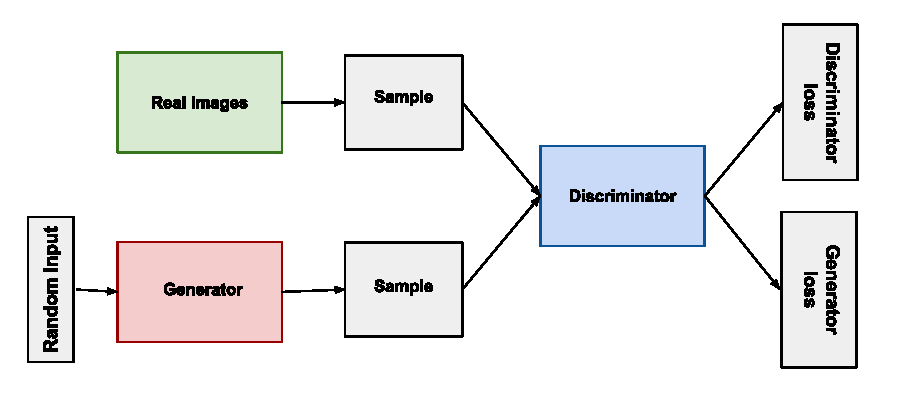
\includegraphics[width=\textwidth]{figure_gan.pdf}
	\caption{Überblick über die GAN-Struktur. Quelle: Google for Developers}
	% https://developers.google.com/machine-learning/gan/gan_structure?hl=de
	\label{fig:gan}
\end{figure}

% Details zum Training
Im Detail wird der Generator durch Minimierung der Log-Wahrscheinlichkeit, dass der Diskriminator die generierten Daten als echt klassifiziert, trainiert. Der Diskriminator wird durch Maximierung dieser Wahrscheinlichkeit trainiert. Dies führt zu einem Gleichgewichtszustand, in dem der Generator realistische Daten erzeugt, die den echten Daten ähneln, und der Diskriminator nicht in der Lage ist, zwischen echten und generierten Daten zu unterscheiden.

Als Verlustfunktion wird die sogenannte \textit{Jensen-Shannon-Divergenz} verwendet, die die Ähnlichkeit zwischen zwei Wahrscheinlichkeitsverteilungen misst:

\begin{equation}
	D_{JS}(P||Q) = \frac{1}{2} D_{KL}(P||M) + \frac{1}{2} D_{KL}(Q||M),
	\label{eq:js-divergence}
\end{equation}

wobei $P$ und $Q$ die beiden Wahrscheinlichkeitsverteilungen und $M$ der Mittelwert der beiden Verteilungen ist.

% Vorteile & Nachteile
Besonders in der Bildgenerierung haben GANs eine hohe Qualität erreicht und sind in der Lage, realistische Bilder zu erzeugen, die von echten Bildern kaum zu unterscheiden sind. GANs sind auch flexibel in Bezug auf die Eingangsdaten und können mit verschiedenen Datentypen wie Bildern, Texten oder Audiodaten arbeiten. Dennoch gibt es einige Nachteile. Beispielsweise kann das Training eines GANs sehr instabil sein, da es schwierig ist, ein Gleichgewicht zwischen Generator und Diskriminator zu finden. Es kann auch zum sogenannten Modus-Kollaps kommen, bei dem der Generator nur eine begrenzte Anzahl von Beispielen erzeugt, da der Diskriminator diese als besonders realistisch bewertet. Der Generator lernt dann, nur diese Beispiele zu reproduzieren, anstatt die gesamte Datenverteilung zu lernen. Darüber hinaus sind GANs sehr rechenaufwändig und erfordern leistungsstarke Hardware, um effizient trainiert zu werden.

\subsection{Diffusionsmodelle} \label{sec:diffusion-models}

% Einleitung, Konzept der Diffusion
Diffusionsmodelle haben in den letzten Jahren zu einem enormen Fortschritt in der Bildgenerierung, insbesondere der Text-to-Image (T2I)-Generierung, geführt. Diese Modelle basieren auf dem Konzept der Diffusion, das aus der Physik stammt. Es beschreibt den Prozess der langsamen Vermischung von Teilchen oder Informationen über die Zeit. Im maschinellen Lernen fand das Konzept erstmals in \parencite{SohlDickstein2015diffusionmodels} Anwendung, mit der Idee, die Struktur von Daten durch Hinzufügen von Rauschen schrittweise aufzulösen und anschließend ein Modell darauf zu trainieren, das ursprüngliche Bild zu rekonstruieren. Seitdem haben sich Diffusionsmodelle als eine neue Klasse von generativen Deep-Learning-Modellen etabliert, die in der Lage sind, noch realistischere Bilder zu generieren als GANs.

% Vorwärts- und Rückwärtsdiffusion als Markov-Ketten
\begin{figure}[h]
	\centering
	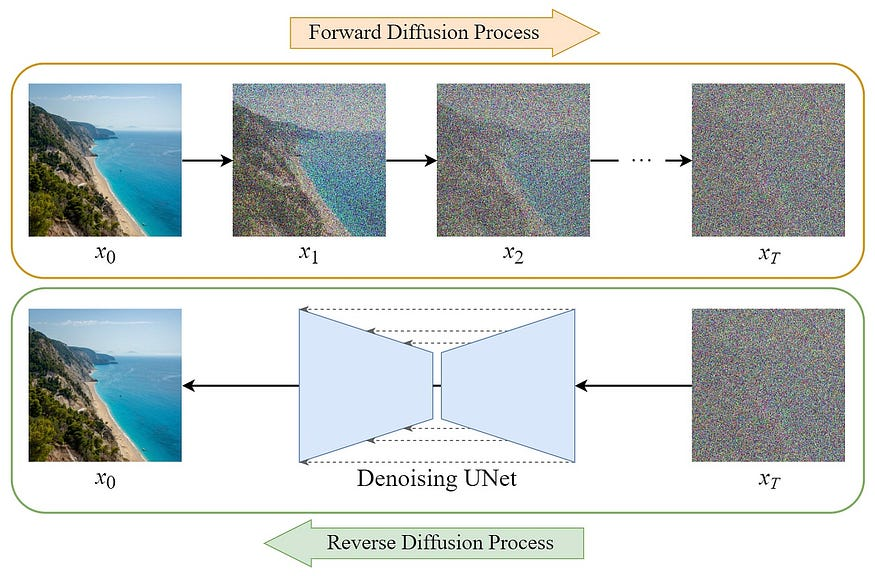
\includegraphics[width=12cm]{figure_stable-diffusion_image.jpg}
	% https://medium.com/@steinsfu/stable-diffusion-clearly-explained-ed008044e07e
	\caption{Darstellung des Vorwärts- und Rückwärtsdiffusion\\in einem Diffusionsmodell.}
	\label{fig:regular-diffusion}
\end{figure}

Das Training von Diffusionsmodelle teilt sich in zwei Phasen auf, die Vorwärts- und die Rückwärtsdiffusion, welche beide als Markov-Ketten modelliert werden können. Markov-Ketten sind stochastische Prozesse, bei denen die zukünftige Entwicklung eines Systems nur von seinem aktuellen Zustand abhängt. Im Bezug auf Diffusionsmodelle repräsentiert jeder Schritt in der Markov-Kette einen Zeitschritt $t$ und die Zustände $x^{(t)}$ sind die Bilder zu diesem Zeitpunkt.

In der Vorwärtsdiffusion wird ein Bild schrittweise durch ein Modell, das Rauschen hinzufügt, in ein verrauschtes Bild umgewandelt. Die Wahrscheinlichkeitsdichte des verrauschten Bildes wird durch die Produktregel der bedingten Wahrscheinlichkeiten berechnet:

\begin{equation}
	q \left( x^{(0 \dots T)} \right) = q \left(x^{(0)}\right)\prod_{t=1}^T q \left(x^{(t)}|x^{(t-1)}\right)
	\label{eq:forward-diffusion}
\end{equation}

In der Rückwärtsdiffusion wird das Modell darauf trainiert, das verrauschte Bild schrittweise in das ursprüngliche Bild zurückzuwandeln. Die Wahrscheinlichkeitsdichte des ursprünglichen Bildes wird durch die Produktregel der bedingten Wahrscheinlichkeiten berechnet:

\begin{equation}
	p \left( x^{(0 \dots T)} \right) = p \left(x^{(T)}\right)\prod_{t=1}^T p \left(x^{(t-1)}|x^{(t)}\right)
	\label{eq:reverse-diffusion}
\end{equation}

Als Verlustfunktion wird die negative Log-Likelihood verwendet, die die Differenz zwischen der tatsächlichen und der modellierten Wahrscheinlichkeitsdichte misst:

\begin{equation}
	Loss = -\log p \left( x^{(0 \dots T)} \right)
	\label{eq:loss-diffusion}
\end{equation}

% Vorteile
Anders als bei GANs gibt es keine direkten adversarialen Optimierungsmechanismen, die zu einem Ungleichgewicht führen können. Es wird stattdessen explizit die Wahrscheinlichkeitsdichte zwischen den realen Daten und den erzeugten Daten minimiert, was zu einem robusteren und stabileren Trainingsprozess führt.

% DALL-E (2) für Text-to-Image
Eine entscheidende Weiterentwicklung der Diffusionsmodelle war die Text-Konditionierung des generativen Prozesses. In \parencite{Ramesh2022dalle2} wurde DALL-E 2 vorgestellt, ein Diffusionsmodell, das in der Lage ist, Bilder aus Textbeschreibungen zu generieren. DALL-E 2 verwendet ein Transformer-Modell, um die Textbeschreibungen in eine latente Repräsentation zu kodieren, die dann als Eingabe für den Diffusionsprozess dient. Auf diese Weise können realistische Bilder erzeugt werden, die den Textbeschreibungen entsprechen. % ?

% Stable Diffusion
Ein besonders einflussreiches Diffusionsmodell ist \textbf{Stable Diffusion} \parencite{Rombach2022stablediffusion}. Die entscheidende Weiterentwicklung von Stable Diffusion liegt darin, dass die Diffusionsprozesse jeweils nur in einem niedrigdimensionalen latenten Raum stattfinden, bevor die Darstellungen wieder in hochauflösende Bilder umgewandelt werden (siehe Abbildung \ref{fig:stable-diffusion}). Dies ermöglicht es, die Komplexität des Modells zu reduzieren und gleichzeitig realistische Bilder zu generieren.

\begin{figure}[h]
	\centering
	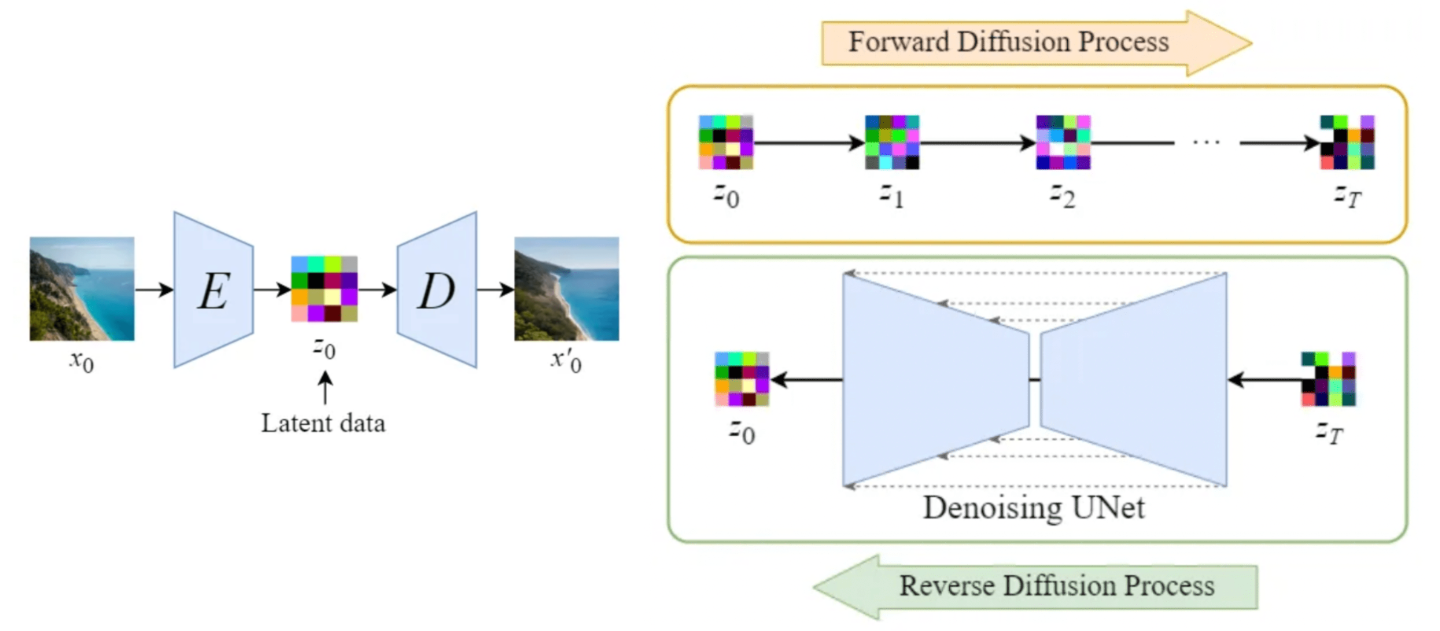
\includegraphics[width=\textwidth]{figure_stable-diffusion_merged.png}
	% https://medium.com/@steinsfu/stable-diffusion-clearly-explained-ed008044e07e
	\caption{Darstellung des Vorwärts- und Rückwärtsdiffusion in Stable Diffusion:\\
		Die	Diffusionsprozesse werden auf die latenten Darstellungen der Bilder\\
		angewendet (rechts), welche vorher mit einem VAE erstellt wurden (links).}
	\label{fig:stable-diffusion}
\end{figure}

\subsection{DA-Fusion} \label{sec:da-fusion}

% Einleitung; Kurze Beschreibung, Versprechen der Methode
In \parencite{Trabucco2023dafusion} wird DA-Fusion, eine auf Stable Diffusion basierende Methode zur Datenaugmentation vorgestellt, die für diese Arbeit von besonderem Interesse ist. Der traditionelle Ansatz der Datenaugmentation, wie in Abschnitt \ref{sec:data-augmentation} beschrieben, hat sich als effektiv erwiesen, um die Generalisierungsfähigkeit von Modellen zu verbessern. Allerdings erfordert dieser Ansatz auch eine gute Intuition in Bezug auf den verwendeten Datensatz, um zu vermeiden, dass Transformationen gewählt werden, durch die Informationen verloren gehen, die für die Aufgabe des zu trainierenden Modells wichtig sind. Wenn beispielsweise Farbinformationen für die Klassifizierung von Blumen wichtig sind, könnte die Datenaugmentation durch zufällige Farbänderungen die Leistung des Modells verschlechtern. Ein weiteres Beispiel sind Objekte, die klein im Bild sind und durch zufällige Ausschnitte des Bildes aus der Sicht des Modells verschwinden können. DA-Fusion hingegen nutzt das Wissen eines vortrainierten Diffusionsmodelle, um den Bildinhalt semantisch zu verstehen und automatisch neue, realistische Variationen zu generieren.

\begin{figure}[h]
	\centering
	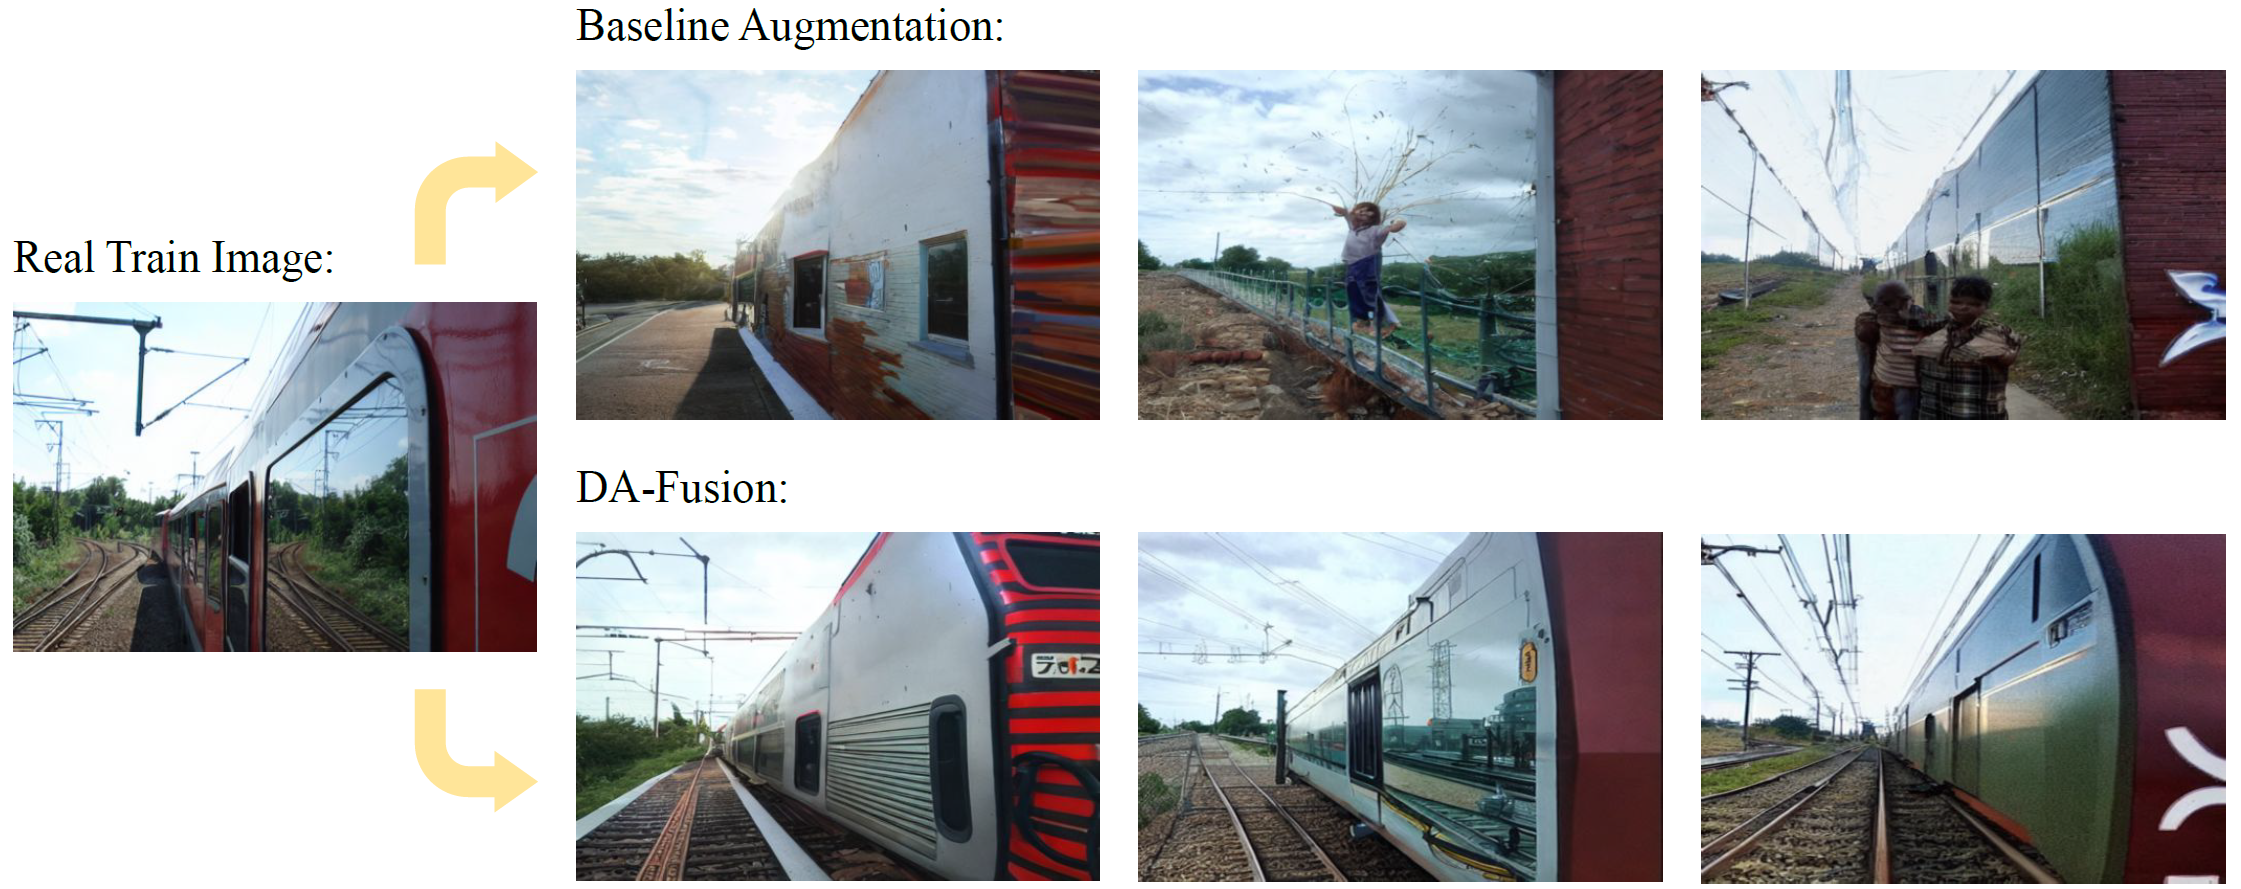
\includegraphics[width=\textwidth]{figure_da-fusion_vs_baseline.png}
	\caption{Vergleich zwischen semantischen Augmentationen aus Baseline-Methode\\
	und DA-Fusion \parencite{Trabucco2023dafusion}.}
	\label{fig:da-fusion}
\end{figure}

% Fine-tuning mit Textual Inversion
Es wird zunächst die Methode Textual Inversion aus \parencite{Gal2022textualinversion} angewendet, um ein vortrainiertes Stable Diffusion-Modell auf den gegebenen Datensatz feinabzustimmen. Dazu wird für jedes Konzept bzw. für jede Klasse ein neues Text-Embedding $y$ als Platzhalter in das Modell integriert, das unter Verwendung von Trainings-Prompts wie "a photo of a <$y$>" und den zugehörigen Bilddaten trainiert wird. Entscheidend ist hier, dass nicht das ganze Diffusionsmodell neu trainiert wird, sondern lediglich neue wörter erlernt werden, welche die spezifischen Konzepte repräsentieren, sodass sich bei der Bildgenerierung weiterhin auf das vortrainierte semantische Wissens des Modells gestützt werden kann.

% Prozess der Datengenerierung
Anschließend können die Bilder augmentiert werden, indem ihnen eine geringe Menge an Rauschen hinzugefügt wird, welches dann durch das feinabgestimmte Modell wieder entfernt werden soll. Hier kommen die selben Text-Prompts zum Einsatz. Auf diese Weise müssen keine völlig neuen Bilder generiert werden, denn die grundlegende Struktur wird durch die ursprünglichen Bilder vorgegeben.

\begin{figure}
	\centering
	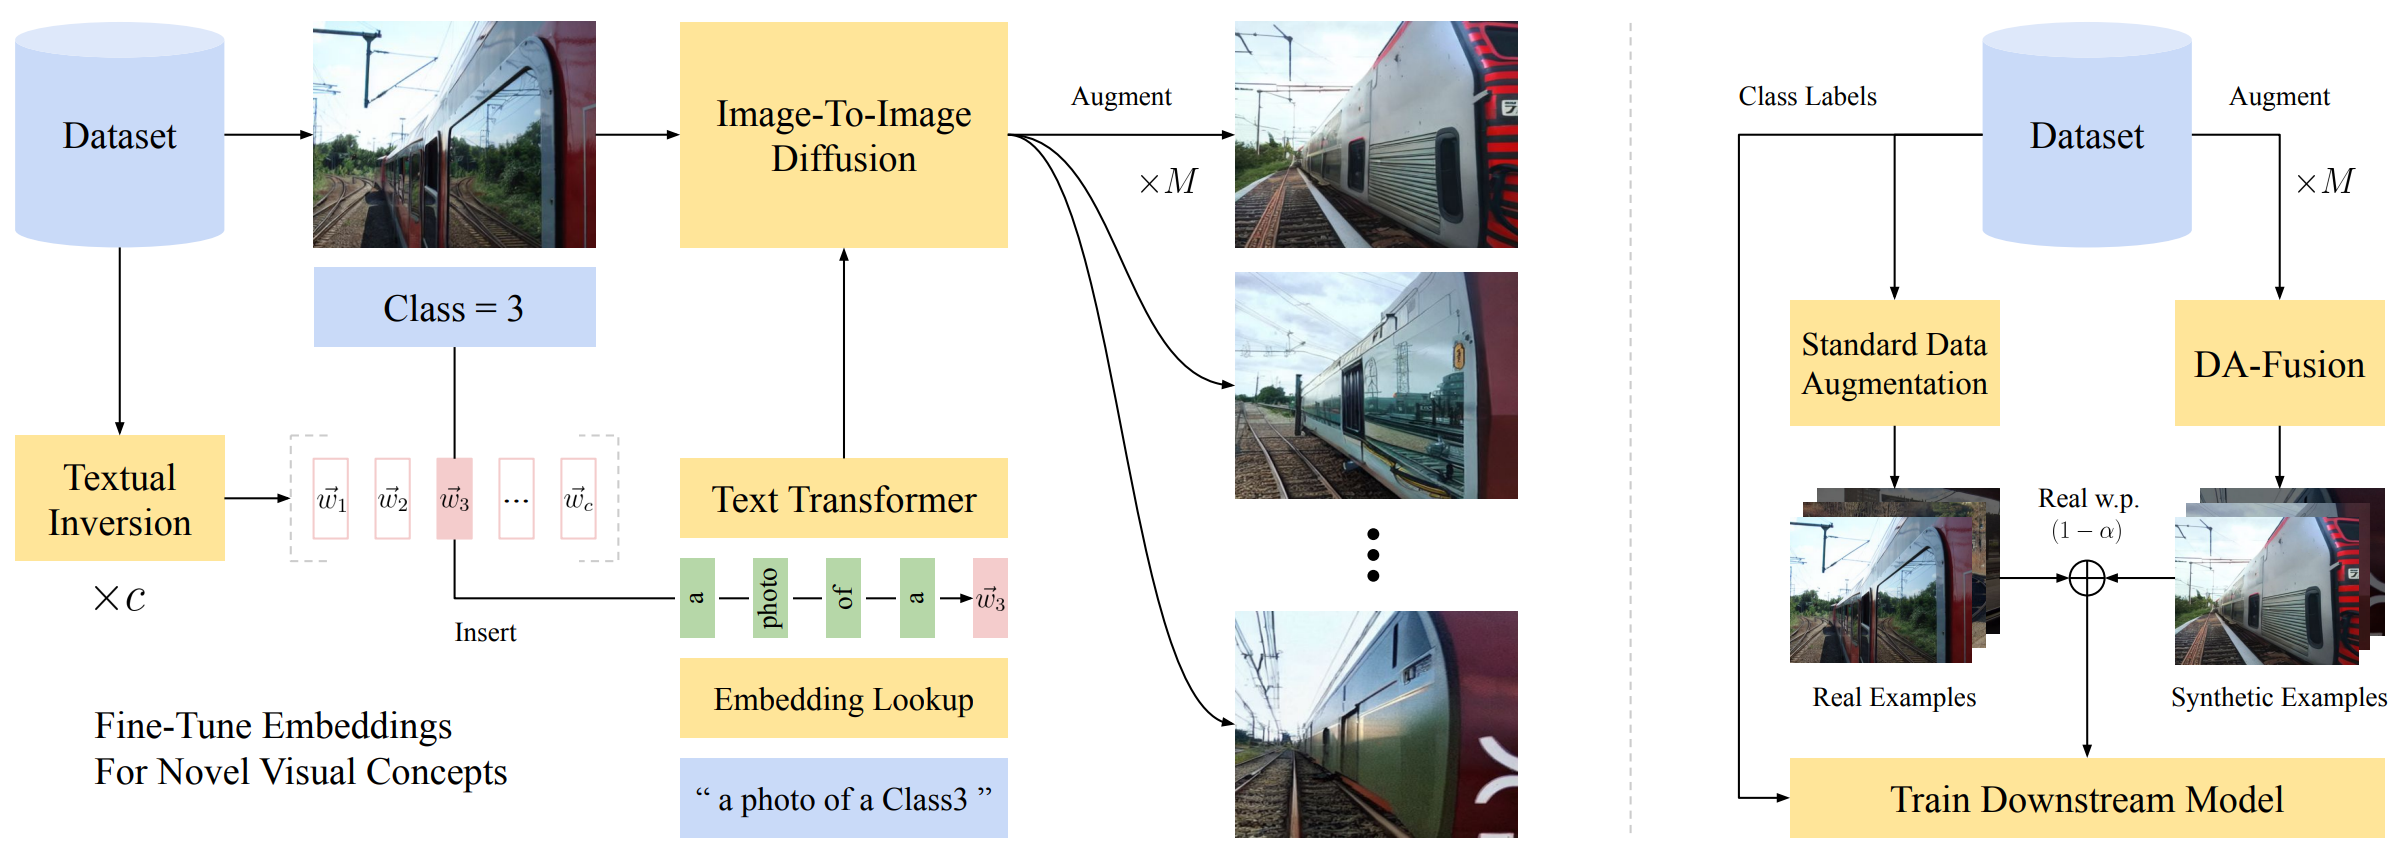
\includegraphics[width=\textwidth]{figure_da-fusion_architecture.png}
	\caption{Überblick über den Prozess zur Datenaugmentation mit\\
	DA-Fusion \parencite{Trabucco2023dafusion}.}
	\label{fig:da-fusion-process}
\end{figure}

% Insertion Timestep als Parameter
Ein Vorteil von DA-Fusion ist die Möglichkeit, den Grad der Augmentation durch die Wahl des Insertion Timesteps zu steuern. Der Insertion Timestep bestimmt, wie weit in den Diffusionsprozess das Bild eingefügt wird und wie stark es dafür vorher verrauscht werden muss. Ein niedriger Timestep führt zu stärkeren Augmentationen, während ein hoher Timestep subtilere Variationen erzeugt.

% DA-Fusion schlägt Prompt-Engineering (Real Guidance) für fine-grained Konzepte, auf die das Diffusion-Modell voraussichtlich noch nicht trainiert wurde

% Ein paar Details zur Implementierung

\section{Klassifikation von Gebrauchsgegenständen für die Recyclingwirtschaft} \label{sec:recycling-classification} %Integration von DA-Fusion und Supervised Contrastive Learning

Der Anwendungsfall, auf den sich diese Arbeit bezieht, ist die Klassifikation verschiedener industrieller Objekte und Gebrauchsgegenstände für die Recyclingwirtschaft. Grundlage dafür ist das Forschungsprojekt “Sensorische \textbf{E}rfassung, automatisierte \textbf{I}dentifikation und \textbf{B}ewertung von \textbf{A}ltteilen anhand von Produktdaten sowie Informationen über bisherige Lieferungen” (EIBA), das im Rahmen der Fördermaßnahme "Ressourceneffiziente Kreislaufwirtschaft \textemdash Innovative Produktkreisläufe (ReziProK)" des Bundesministeriums für Bildung und Forschung entstand \parencite{Wagner2022reziprok}. Neben dem Fraunhofer-IPK waren auch die Technische Universität Berlin, die Deutsche Akademie der Technikwissenschaften (acatech), sowie die Circular Economy Solutions GmbH beteiligt.

Das Ziel des Projekts war die Entwicklung eines KI-gestützten Systems, welches Daten aus verschiedenen digitalen Sensoren, sowie Kontextdaten aus dem Geschäftsprozess verarbeitet, um bei der Identifikation, Inspektion und Sortierung von Altteilen zu unterstützen. Dabei betont das Projekt die Rolle der KI zur \textit{Unterstützung} des Menschen, nicht zur vollständigen Automatisierung \parencite{Wagner2022reziprok}. In Abbildung \ref{fig:eiba-process} wird veranschaulicht, wie sich das System in die genannten Prozesse integriert.

\begin{figure}[h]
	\centering
	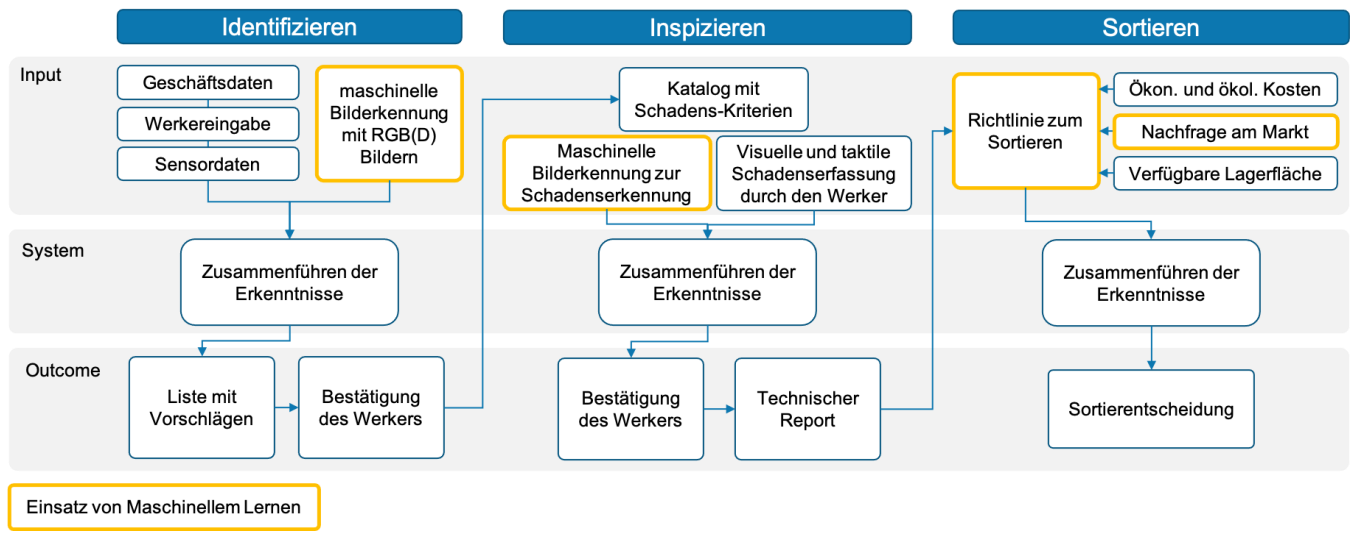
\includegraphics[width=\textwidth]{figure_eiba_process.png}
	\caption{Integration des in EIBA entwickelten KI-gestützten Systems\\
	in den Prozess der Indentifikation, Inspektion und Sortierung\\
	von Altteilen \parencite{Wagner2022reziprok}.}
	\label{fig:eiba-process}
\end{figure}

Viele der Altteile sind sehr ähnlich und erfordern Expertenwissen, um sie korrekt zu identifizieren und den Beschädigungsgrad zu bewerten. Die Beschriftungen und Barcodes sind oft nicht mehr lesbar, sodass die Identifikation rein visuell erfolgen muss \parencite{Wagner2022reziprok}. Hier setzt das KI-System an, um den Menschen zu unterstützen. Es werden dafür multimodale Sensordaten verwendet, unter anderem Tiefenkameras (RGB-D) und eine Waage zur Erfassung des Gewichts zum Einsatz. In Abbildung \ref{fig:eiba-interface} ist die Mensch-Maschine-Schnittstelle einer mobilen Teststation des Systems dargestellt.

\begin{figure}[h]
	\centering
	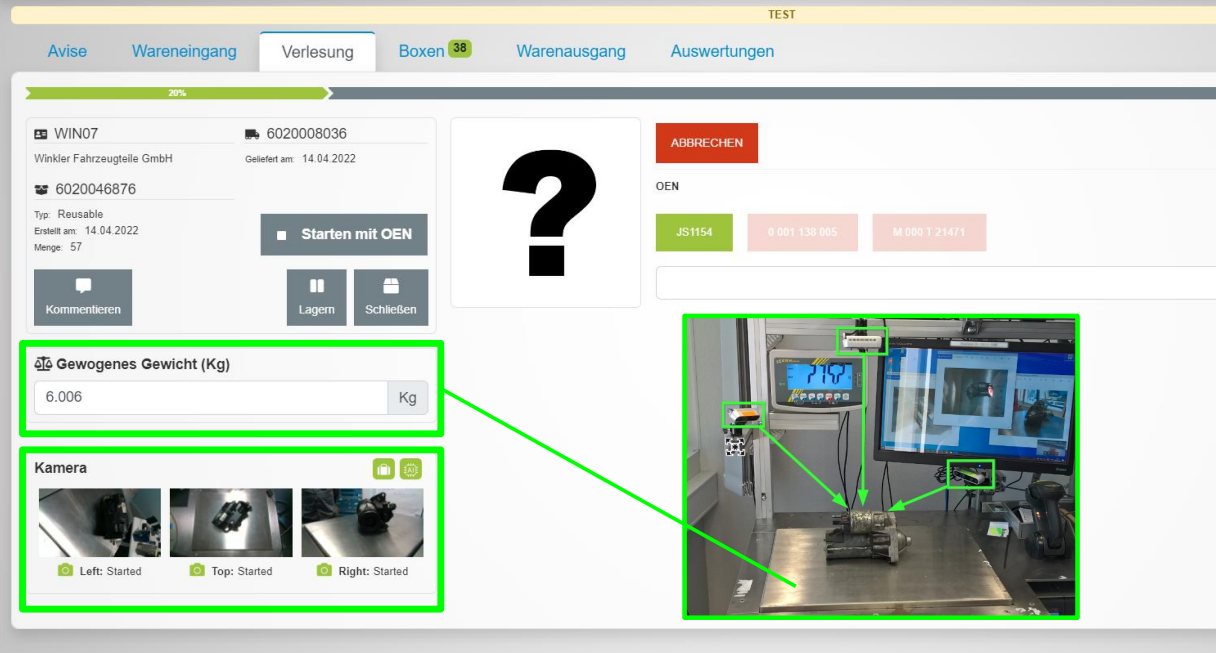
\includegraphics[width=\textwidth]{figure_eiba_interface.png}
	\caption{Die Mensch-Maschine-Schnittstelle des Systems \parencite{Wagner2022reziprok}.}
	\label{fig:eiba-interface}
\end{figure}

% Ergebnisse vielversprechend, aber vorerst nur im Labor; Generalisierung verbessern
Das System wurde am Beispiel von gebrauchten Fahrzeugteilen entwickelt und konnte bei Tests basierend auf Bilddaten von ca. 1.400 Altteilen über 98\% Accuracy erreichen \parencite{ReziProK2019eiba}. Da die Tests jedoch unter Laborbedingungen stattfanden, wird weiterhin nach Möglichkeiten gesucht, die Generalisierungsfähigkeit des Modells zu verbessern. Insbesondere die Klassifikation von Objekten in verschiedenen Gebrauchszuständen, wie z.B. beschädigte oder verschmutzte Teile, stellt eine Herausforderung dar.

In den vorherigen Abschnitten wurden verschiedene Methoden zur Verbesserung der Generalisierungsfähigkeit und Robustheit von Modellen vorgestellt. Sowohl das Contrastive Learning als auch die synthetische Datengenerierung bzw. Datenaugmentation konnten jeweils vielversprechende Ergebnisse erzielen. In dieser Arbeit wird nun ein Ansatz zur Kombination beider Methoden vorgestellt, welcher eine neuartige Verwendung von synthetischen Daten im Contrastive Learning ermöglichen könnte.

\subsection{Herausforderungen bei der Generierung synthetischer Daten} \label{sec:challenges-synt-data}

Zunächst soll auf eine Reihe von Herausforderungen bei der Generierung synthetischer Daten aufmerksam gemacht werden, insbesondere im Kontext des vorgestellten Anwendungsfalls. Für herkömmliche Methoden zur Bildgenerierung, wie GANs oder Diffusionsmodelle, ergeben sich hier nämlich spezielle Herausforderungen:

% Herausforderungen
\begin{itemize}
	\item Die Objekte weisen teilweise eine sehr hohe \textbf{Komplexität} auf, etwa bei Motoren oder Generatoren mit vielen Details. Auch moderne Methoden zur Bildgenerierung können daran scheitern, diese Details korrekt zu erlenrn und zu reproduzieren \textemdash insbesondere, wenn nur wenige Beispielbilder gegeben sind.
	\item Es gibt oft nur \textbf{feine Unterschiede} zwischen den Klassen, die es zu berücksichtigen gilt. Sind die generierten Daten nicht akkurat genug, kann es zu Fehlklassifikationen kommen.
	\item Auf Grund des Multiview-Setups haben die Bilder nur \textbf{wenig Variation}, vor allem in den Hintergründen. Auch die Objekte selbst sind zwar aus verschiedenen Perspektiven aufgenommen, bieten aber pro Klasse nicht viel Variation in Bezug auf die Beschaffenheit, die Farbe, usw.
\end{itemize}

% Anforderungen
Es ergeben sich also hohe Anforderungen an die Generierung der synthetischen Daten. Einerseits muss die Genauigkeit der generierten Daten gewährleistet sein, um die Klassifikation der Modelle nicht zu beeinträchtigen. Trotzdem muss genügend Variation ermöglicht werden, um die Generalisierungsfähigkeit der Modelle zu verbessern.

\subsection{Synthetische Daten als negativ-Beispiele im Contrastive Learning} \label{sec:synt-ood-contrastive}

% Herausforderungen -> Forschungslücke ?
Aus den spezifischen Herausforderungen bei der Generierung synthetischer Daten, zusammen mit den Besonderheiten des Contrastive Learning, ergibt sich eine interessante Forschungslücke: Ist es möglich, auch aus \textit{mangelhaften} synthetischen Daten zu lernen, wenn sie ausschließlich als negativ-Beispiele im Contrastive Learning verwendet werden? Genauer, lässt sich so die Leistung eines Modells bei der Klassifikation von echten Daten verbessern und gleichzeitig die Robustheit gegenüber OOD-Daten erhöhen?

% SimCLR profitierte besonders von hard negatives, um gute Repräsentationen zu lernen
	% Synt Daten dürfen also nicht zu entfernt sein: CL lernt vor allem aus HARD Negatives
Die bisherigen Erfolge von Contrastive Learning, insbesondere von SimCLR, zeigen, dass das Modell besonders von Hard Negatives profitiert \parencite{Chen2020simclr}, also von unähnlichen Beispielen, die aber nur schwer zu unterscheiden sind. Auch \parencite{Jiang2024supconhardnegatives} baut auf dieser Erkenntnis auf, jedoch ohne Verwendung von synthetischen Daten. Die synthetischen Daten dürften also nicht zu weit entfernt von den echten Daten sein, um die Repräsentationen zu verbessern. Sie könnten daher als \textit{Near OOD}-Beispiele bezeichnet werden, wobei sie noch OOD genug sein müssen, um die Distanz zwischen den In-Distribution und OOD-Daten zu maximieren. Ob sich diese synthetischen Near OOD-Daten tatsächlich als gute Hard Negatives herausstellen, wird in dieser Arbeit untersucht.

% StableRep: Synthetische Diffusion-Daten im Contrastive Learning, aber nur normale ID-Beispiele
	% Stable Diffusion "off-the-shelf" ist nicht akkurat genug
		% Objekte zu komplex
		% Zu ähnlich; feine Unterschiede
	% Auch die gleichbleibenden Hintergründe sind fatal
	% Außerdem: Unsupervised

% Was wenn: Anstatt Negatives aus Nähe im Darstellungsraum zu samplen, Near OOD-Augmentationen aus Anchor-Klasse?

\subsection{Integration von DA-Fusion und Supervised Contrastive Learning} \label{sec:da-fusion-supcon}

% DA-Fusion zur Generierung von ID- und Near OOD-Daten
...

% Einfach den strength-Parameter der DA-Fusion-Augmentationen erhöhen

% Bei der Generierung die Maske verwenden, damit die Hintergründe gleich bleiben

% Supervised Contrastive Learning mit eigener Sampling-Strategie für Near OOD-Negatives

% Potenzielle Vorteile
	% Bessere Generalisierung trotz Limitationen in der Datengenerierung
		% OOD-Augmentationen müssen an sich keine spezifischen Klassen akkurat repräsentieren, sind aber dennoch nah genug an den echten Daten, um dessen Repräsentationen zu verbessern
	% Bessere OOD-Detektion
		% OOD-Detection profitiert von einer guten Repräsentation der Daten, um die Distanz zwischen In-Distribution und OOD-Daten zu maximieren
% Potenzielle Herausforderungen
	% ...